% Векторизация циклов с нерегулярным количеством итераций.
\subsection{Векторизация гнезд циклов с нерегулярным количеством итераций}

Рассмотренный в разделе \ref{sec:text_4_vec_riemann} программный контекст римановского решателя относится к кодам моделирования физических процессов.
Для таких кодов характерно медленное изменение физических величин при переходе от одной расчетной ячейке к другой.
Это свойство физических расчетных кодов позволяет применять такие подходы к векторизации как проверка масок на пустоту (раздел~\ref{sec:text_4_vec_check_mask}), удаление маловероятных регионов (раздел~\ref{sec:text_4_loc_branch}) и позволяет эффективно выполнять векторизацию гнезд циклов с непостоянным количеством итераций.
В этом разделе рассмотрим принципиально другой тип контекста, в котором на двух соседних итерациях плоского цикла невозможно пресказать состояние условия, что приводит к возникновению гнезд циклов с нерегулярным количеством итераций \cite{Rybakov2019VecIrr,Rybakov2018VecNest,Shabanov2019VecSci}.
Такой программный контекст будем рассматривать на примере сортировки Шелла, которая является крайне неудобной для векторизации.

\subsubsection{Описание сортировки Шелла}

Сортировка Шелла \cite{Knut1994} представляет собой расширение сортировки вставками, которое работает быстрее, так как позволяет на ранних этапах упорядочить далеко расположенные друг от друга элементы массива, это приводит к тому, что массив становится частично упорядоченным.
Во время сортировки Шелла выполняется последовательная сортировка подмассивов основного массива, являющихся срезами, при этом шаг среза постоянно уменьшается и на завершающем этапе выполняется обычная сортировка вставками (это соответствует срезу массива с шагом 1).
Выполнение сортировки срезов массива с большими шагами облегчает сортировку срезов с меньшими значениями шага, эффективность сортировки существенно зависит от выбранной последовательности шагов.

В литературе описано множество существующих последовательностей, из которых мы будем анализировать лишь некоторые, представленные в таблице~\ref{tbl:text_4_vec_irreg_steps}:

\begin{table}
\centering
\caption{Различные последовательности шагов, используемые в сортировке Шелла.}
\bigskip
\label{tbl:text_4_vec_irreg_steps}
\begin{tabular}{ | c | c | }
  \hline
  Последовательность & Формула \\ \hline\hline
  \makecell{Последовательность \\ Шелла} & $k_1 = \lfloor \frac{N}{2} \rfloor, \ k_i = \lfloor \frac{k_{i-1}}{2} \rfloor, \ k_t = 1$ \\ \hline
  \makecell{Последовательность \\ Хиббарда \cite{seqHibbard}} & $2^i - 1 \le N$, $i \in \mathbb{N}$ \\ \hline
  \makecell{Последовательность \\ Пратта \cite{seqPratt}} & $2^i \cdot 3^j \le \frac{N}{2}$, $i \in \mathbb{N}$, $j \in \mathbb{Z}_{\ge 0}$ \\ \hline
  \makecell{Последовательность \\ Седжвика \cite{seqSadgwick}} & $k_i = \begin{cases} 9 \cdot 2^i - 9 \cdot 2^{\frac{i}{2}} + 1, \ i = 2m, \ m \in \mathbb{Z}_{\ge 0} \\ 8 \cdot 2^i - 6 \cdot 2^{\frac{i + 1}{2}}, \ i = 2m + 1, \ m \in \mathbb{Z}_{\ge 0} \end{cases}$ \\ \hline
\end{tabular}
\end{table}

Реализация сортировки Шелла состоит из гнезда циклов, содержащего три цикла.
Внешний цикл выполняется по всем шагам из используемой последовательности шагов, начиная с максимального и заканчивая единицей.
Два внутренних цикла осуществляют сортировку всех подмассивов, являющихся срезами исходного массива с текущим шагом $k$ (листинг~\ref{lst:text_4_vec_irreg_shell}).

\begin{lstlisting}[caption={Реализация сортировки Шелла.},label={lst:text_4_vec_irreg_shell}]
void shell_sort(float* m, int n, int* ks, int k_ind)
{
    int i, j, k;

    for (k = ks[k_ind]; k > 0; k = ks[--k_ind])
    {
        for (i = k; i < n; i++)
        {
            float t = m[i];

            for (j = i; j >= k; j -= k)
            {
                if (t < m[j - k])
                {
                    m[j] = m[j - k];
                }
                else
                {
                    break;
                }
            }

            m[j] = t;
        }
    }
}
\end{lstlisting}

\subsubsection{Векторизация сортировки Шелла}

Рассмотрим возможности по векторизации сортировки Шелла для массива вещественных значений типа float (вектор AVX-512 содержит 16 таких значений).
Самый вложенный цикл (цикл с счетчиком $j$, будем называть его просто внутренним) выполняет сортировку одного среза, состоящего из элементов массива, с расстоянием $k$ между соседними элементами.
Внутренний цикл не может быть векторизован без выполнения дополнительных модификаций кода, так как между записью элемента \texttt{m[j]} и чтением элемента \texttt{m[j - k]} существует межитерационная зависимость.
Однако, можно заметить, что две итерации среднего по вложенности цикла (цикла с индуктивной переменной $i$, будем называть его промежуточным) с номерами $i_1$ и $i_2$ не пересекаются по данным и могут быть выполнены параллельно при выполнении условия $|i_1 - i_2| < k$.
Выполним декомпозицию сортировки Шелла для того, чтобы можно было явно выделить ядро, поддающееся векторизации.

На рис.~\ref{fig:text_4_vec_irreg_code_decomp} представлена схема декомпозиции алгоритма сортировки Шелла, в котором явно выделены участки с разной шириной векторизации.
Сначала выделен блок для шагов $k \ge 16$.
Для этих значений шагов можно параллельно выполнять 16 соседних итераций промежуточного цикла, при этом достигается максимальная плотность векторизации (показано зеленым цветом на схеме).

\begin{figure}[ht]
	\centering
	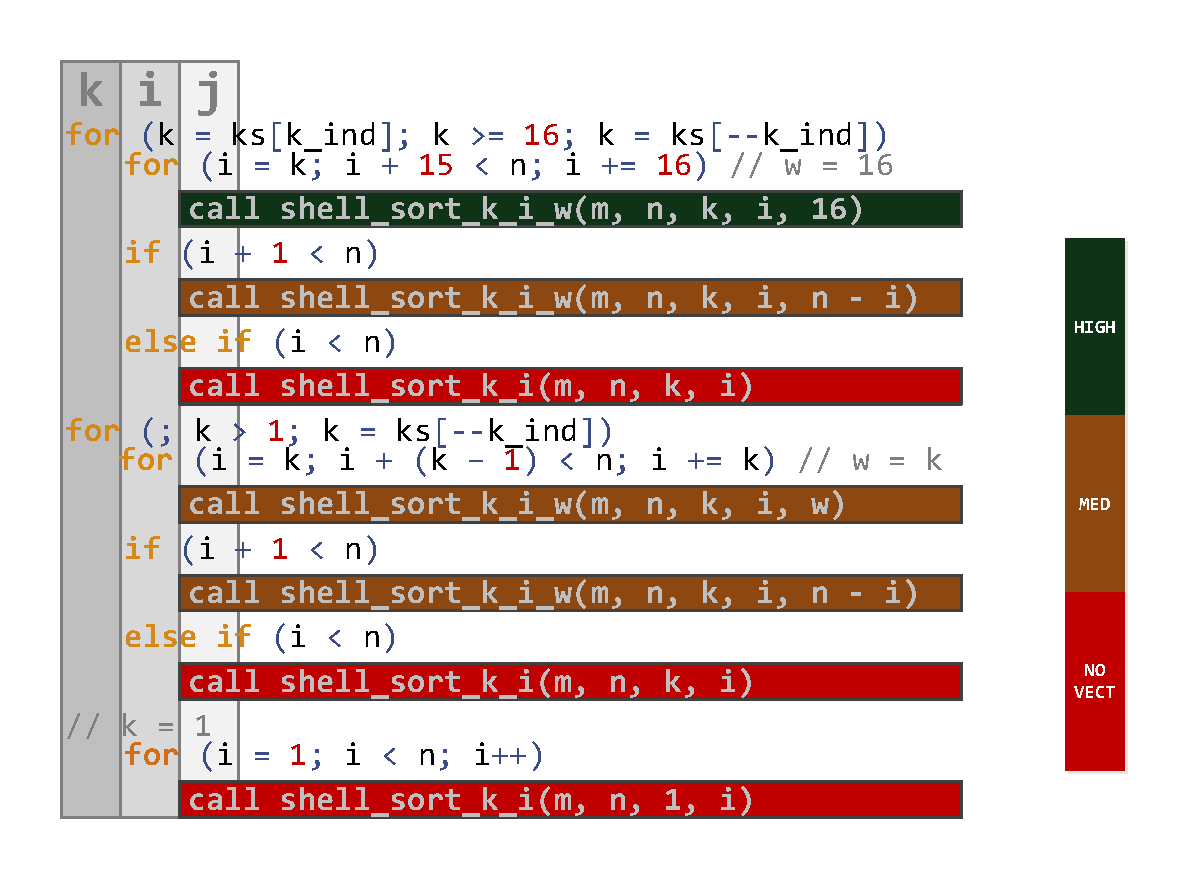
\includegraphics[width=0.8\textwidth]{./pics/text_4_vec_irreg/code_decomp.pdf}
	\caption{Декомпозиция сортировки Шелла для выделения векторизуемых участков кода.}
	\label{fig:text_4_vec_irreg_code_decomp}
\end{figure}

Все итерации промежуточного цикла разбиваются на группы по 16 соседних итераций и остаток, который векторизуется с шириной меньше 16 (показано желтым цветом, а в том случае, когда остаток состоит всего из одной итерации, то векторизация не требуется, что показано красным цветом на схеме).
Далее рассматривается блок значений шагов $1 < k < 16$.
При этих значениях ширина векторизации всегда меньше 16, к тому же, как и в предыдущем блоке, возможно появление невекторизуемого остатка.

В последнюю очередь рассматривается невекторизуемая финальная сортировка вставками для $k = 1$.
Наличие участков кода с шириной векторизации менее 16 приводит к неоптимальному результирующему коду, однако есть более опасная причина низкой эффективности векторизации.

Функция \texttt{shell\_sort\_k\_i\_w}, появившаяся после декомпозиции алгоритма сортировки Шелла, содержит реализацию сортировки $w$ соседних срезов массива, взятых с шагом $k$.
При этом количество итераций внутреннего цикла этой функции является неизвестным.
Более того, количество итераций внутреннего цикла при сортировке одного среза никак не связано с количеством итераций внутреннего цикла при сортировке соседнего среза.
Это является существенной проблемой при попытке объединить код сортировки соседних срезов, используя векторные инструкции.

Для такого объединения необходимо переписать код сортировки среза в предикатной форме, после чего заменить все инструкции векторными аналогами, а предикаты –- векторными масками (см. рис.~\ref{fig:text_4_vec_irreg_shell_cfg}).
При этом если до векторизации внутренний цикл завершал работу при обращении предиката в false, то после векторизации внутренний цикл завершит работу, только если все элементы соответствующей векторной маски обнулятся.
Таким образом, количество итераций векторизованного внутреннего цикла равно максимальному количеству итераций всех объединяемых $w$ циклов.

\begin{figure}[ht]
	\centering
	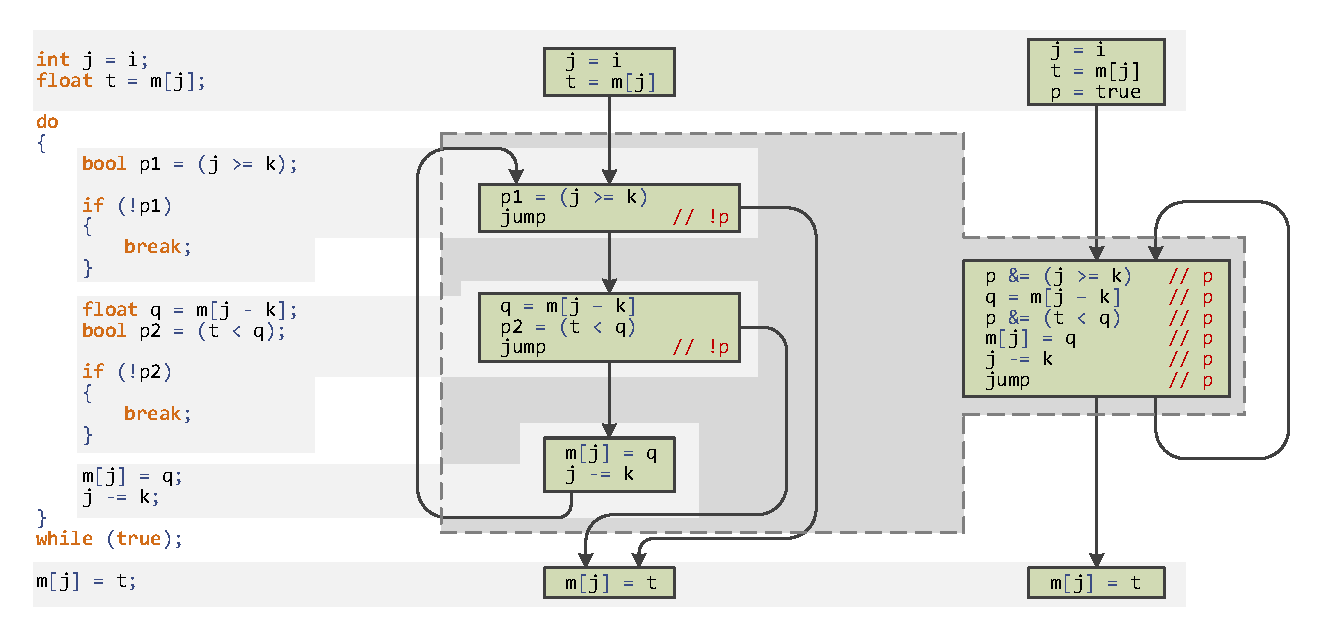
\includegraphics[width=1.0\textwidth]{./pics/text_4_vec_irreg/shell_cfg.pdf}
	\caption{Схема перевода тела внутреннего цикла сортировки Шелла в предикатную форму.}
	\label{fig:text_4_vec_irreg_shell_cfg}
\end{figure}

Если значения количества итераций соседних объединяемых циклов различаются сильно (а для сортировки Шелла это утверждение верно), то мы получаем потерю эффективности векторизации из за низкой плотности масок векторных инструкций (то есть малый процент элементов векторов на самом деле обрабатывается при выполнении векторной операции).
Такой негативный эффект при векторизации гнезд циклов характерен для дискретных задач, в том числе для задач сортировки, поиска, комбинаторного перебора с отсечением ветвей и других.

Для задач численного моделирования физических процессов наоборот данный эффект практически незаметен, профиль исполнения отдельных участков программного кода меняется не сильно при небольших изменениях входных данных.

Векторизованная версия ядра сортировки Шелла представлена на листинге~\ref{lst:text_4_vec_irreg_shell_vec}:

\begin{lstlisting}[caption={Векторизованный вариант ядра сортировки Шелла.},label={lst:text_4_vec_irreg_shell_vec}]
void shell_sort_k_i_w(float *m, int n, int k, int i, int w)
{
    int j = i;
    __mmask16 ini_mask = ((unsigned int)0xFFFF) >> (16 - w);
    __mmask16 mask = ini_mask;
    __m512i ind_j = _mm512_add_epi32(_mm512_set1_epi32(i),
                                     ind_straight);
    __m512 t, q;

    t = _mm512_mask_load_ps(t, mask, &m[j]);

    do
    {
        mask = mask & _mm512_mask_cmp_epi32_mask(mask, ind_j, ind_k,
                                                 _MM_CMPINT_GE);
        q = _mm512_mask_load_ps(q, mask, &m[j - k]);
        mask = mask & _mm512_mask_cmp_ps_mask(mask, t, q,
                                              _MM_CMPINT_LT);
          _mm512_mask_store_ps(&m[j], mask, q);
        ind_j = _mm512_mask_sub_epi32(ind_j, mask, ind_j, ind_k);
        j -= k;
    }
    while (mask != 0x0);

    _mm512_mask_i32scatter_ps(m, ini_mask, ind_j, t, _MM_SCALE_4);
}
\end{lstlisting}

Также стоит обратить внимание на появившуюся в векторном коде операцию scatter (листинг~\ref{lst:text_4_vec_irreg_shell_vec}, строка 25) множественной записи данных в память с произвольными смещениями относительно базового адреса.
Эта команда появилась как векторный аналог операции записи в память из оригинального кода (листинг~\ref{lst:text_4_vec_irreg_shell}, строка 23) ввиду той же причины –- нерегулярности количества итераций внутреннего цикла.
Стоит отметить, что команды scatter являются крайне медленными, что также является причиной снижения эффективности векторизации.

Кроме обозначенной команды scatter в векторизованном коде присутствуют другие команды обращения в память (листинг~\ref{lst:text_4_vec_irreg_shell_vec}, строки 10, 16, 19).
Это масочные команды чтения и записи по последовательным адресам, реализованные интринсиками \texttt{\_mm512\_mask\_load\_ps} и \texttt{\_mm512\_mask\_store\_ps}, которые раскрываются в операции невыровненного обращения в память vmovups.

В этом случае нельзя использовать выровненные операции обращения в память, так как в общем случае адреса обращения в данных командах конечно не являются выровненными.
В микропроцессорах Intel Xeon Phi KNL и Intel Xeon Skylake скорость обращения в память команд vmovaps не отличается от скорости обращения vmovups при условии выровненного обращения, поэтому компилятор icc вовсе не генерирует инструкции vmovaps \cite{MOVUPSintel}.
Таким образом, при невыполнении условия выровненности адресов вместо аварийного завершения мы получаем снижение производительности программы, однако это снижение не сравнимо с медленной работой инструкций gather и scatter.

\subsubsection{Вычисление теоретического ускорения при векторизации сортировки Шелла}

В этом разделе произведем вычисление теоретического ускорения, которое может быть достигнуто при векторизации сортировки Шелла предложенным способом. 
При этом под теоретическим ускорением будем подразумевать просто отношение количества итераций внутреннего цикла невекторизованной версии к количеству итераций внутреннего цикла в оптимизированной векторизованной версии кода.
Определим это ускорение более формально.

Сначала рассмотрим невекторизованный код.
Обозначим через $T(k, i)$ количество итераций внутреннего цикла при фиксированных $k$ и $i$. 
Тогда не составляет труда вычислить общее количество итераций внутреннего цикла при выполнении сортировки (обозначим эту велечину через $T$).
\begin{equation}
	T = \sum_{k \in ks}{\sum_{i = k}^{n - 1}{T(k, i)}}
\end{equation}

Теперь рассмотрим векторизованную версию кода. 
Аналогично обозначим через $T_v(k,i)$ количество итераций внутреннего цикла при фиксированных $k$ и $i$. 
Нам известно, что ширина векторизации не может превышать $k$ (из-за зависимостей по обращению к массиву), и 16 (размер вектора), то есть $w(k) = \min(k, 16)$. 
При этом весь диапазон значений $i$ от $k$ до $n - 1$, длина которого равна $n - k$ разбивается на $\lfloor \frac{n - k}{w(k)} \rfloor$ групп по $w$ элементов в каждой, и количество итераций в векторизованном цикле, соответствующем каждой группе равно максимальному значению из количеств итераций невекторизованных циклов, объединяемых в данный векторизованный цикл. 
С учетом векторизации хвостовой части цикла, получим следующую формулу для общего количества итераций векторизованного внутреннего цикла.
\begin{equation}
	T_v = \sum_{k \in ks}
	{
		\left(
			\left(
				\sum_{g = 0}^{G(k) - 1}{\max_{i = k + w(k)g}^{k + w(k)(g + 1) - 1}{I(k, i)}}
			\right)
			+ \max_{i = k + w(k)G(k)}^{n - 1}{I(k, i)}
		\right)
	}
\end{equation}

где $w(k) = \min(k, 16)$, $G(k) = \lfloor \frac{n - k}{w(k)} \rfloor$. 
Значения $T = T(n)$ и $T_v = T_v(n)$ были вычислены при сортировке псевдослучайных массивов с количеством элементов от 10 тыс. до 2 млн для каждой из последовательностей шагов Хиббарда, Пратта и Сэджвика. 
На основе этого вычислялось теоретическое ускорение $s(n) = T(n)/T_v(n)$. 
Кроме того, аналогичные характеристики рассчитывались и без учета шага $k = 1$ (эти величины обозначены $T'(n)$, $T'_v(n)$ и $s'(n)$ соответственно). 
Полученные результаты сравнивались с результатами экспериментальных запусков на микропроцессоре Intel Xeon Phi 7290 KNL.

\subsubsection{Экспериментальные результаты эффективности векторизации сортировки Шелла}

\begin{figure}[ht]
	\centering
	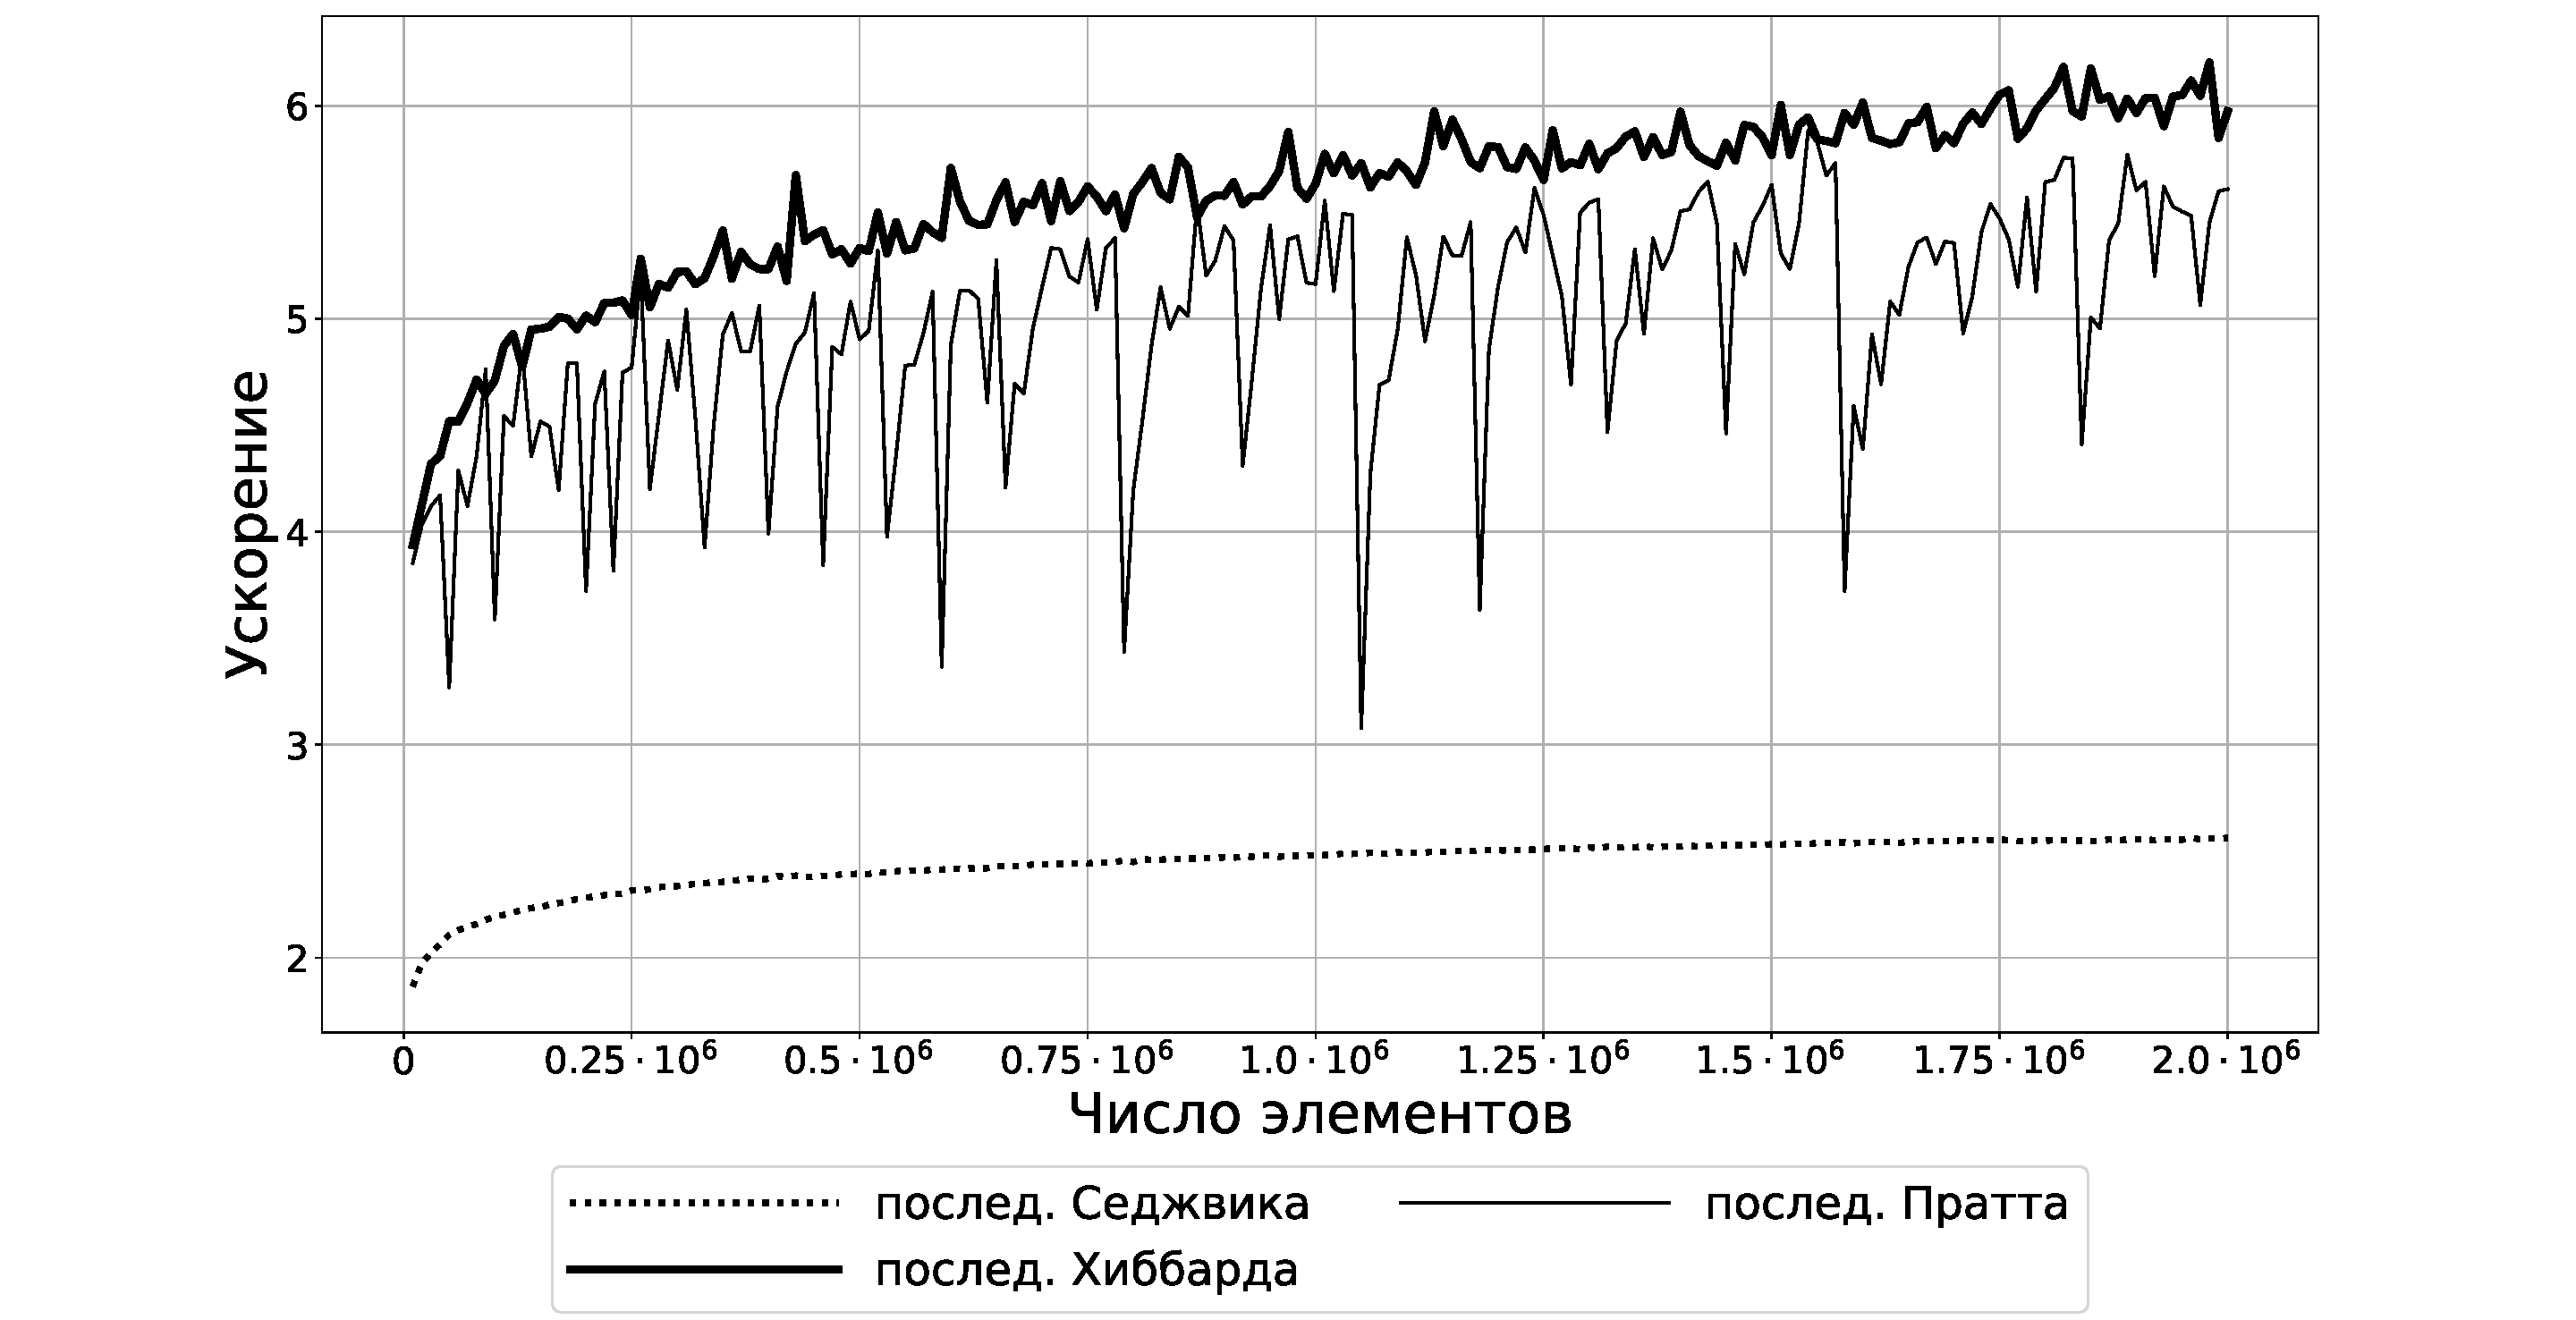
\includegraphics[width=1.0\textwidth]{./pics/text_4_vec_irreg/theoretical_eff.pdf}
	\caption{Сравнение теоретического ускорения векторизованной версии сортировки Шелла для различных
последовательностей шагов.}
	\label{fig:text_4_vec_irreg_theoretical_eff}
\end{figure}

Для проведения экспериментов были использованы две версии исходного кода: неоптимизированная функция сортировки и реализованная с помощью функций-инстринсиков.
Обе версии сортировки были собраны компилятором icc с уровнем оптимизаии -O3 и с разрешением генерировать инструкции AVX-512 (-xmic-avx512) для микропроцессора Intel Xeon Phi KNL.
Тестовые запуски и замер времени исполнения выполнялись на одном вычислительном узле суперкомпьютера МВС-10П, на сегменте, базирующимся на микропроцессорах Intel Xeon Phi 7290.

На рисунках \ref{fig:text_4_vec_irreg_theoretical_eff} и \ref{fig:text_4_vec_irreg_experimental_eff} представлены результаты теоретических оценок и экспериментальных запусков, исходя из которых получены теоретическое и экспериментальное ускорение сортировки Шелла для последовательностей шагов Шелла, Хиббарда и Сэджвика:

\begin{figure}[ht]
	\centering
	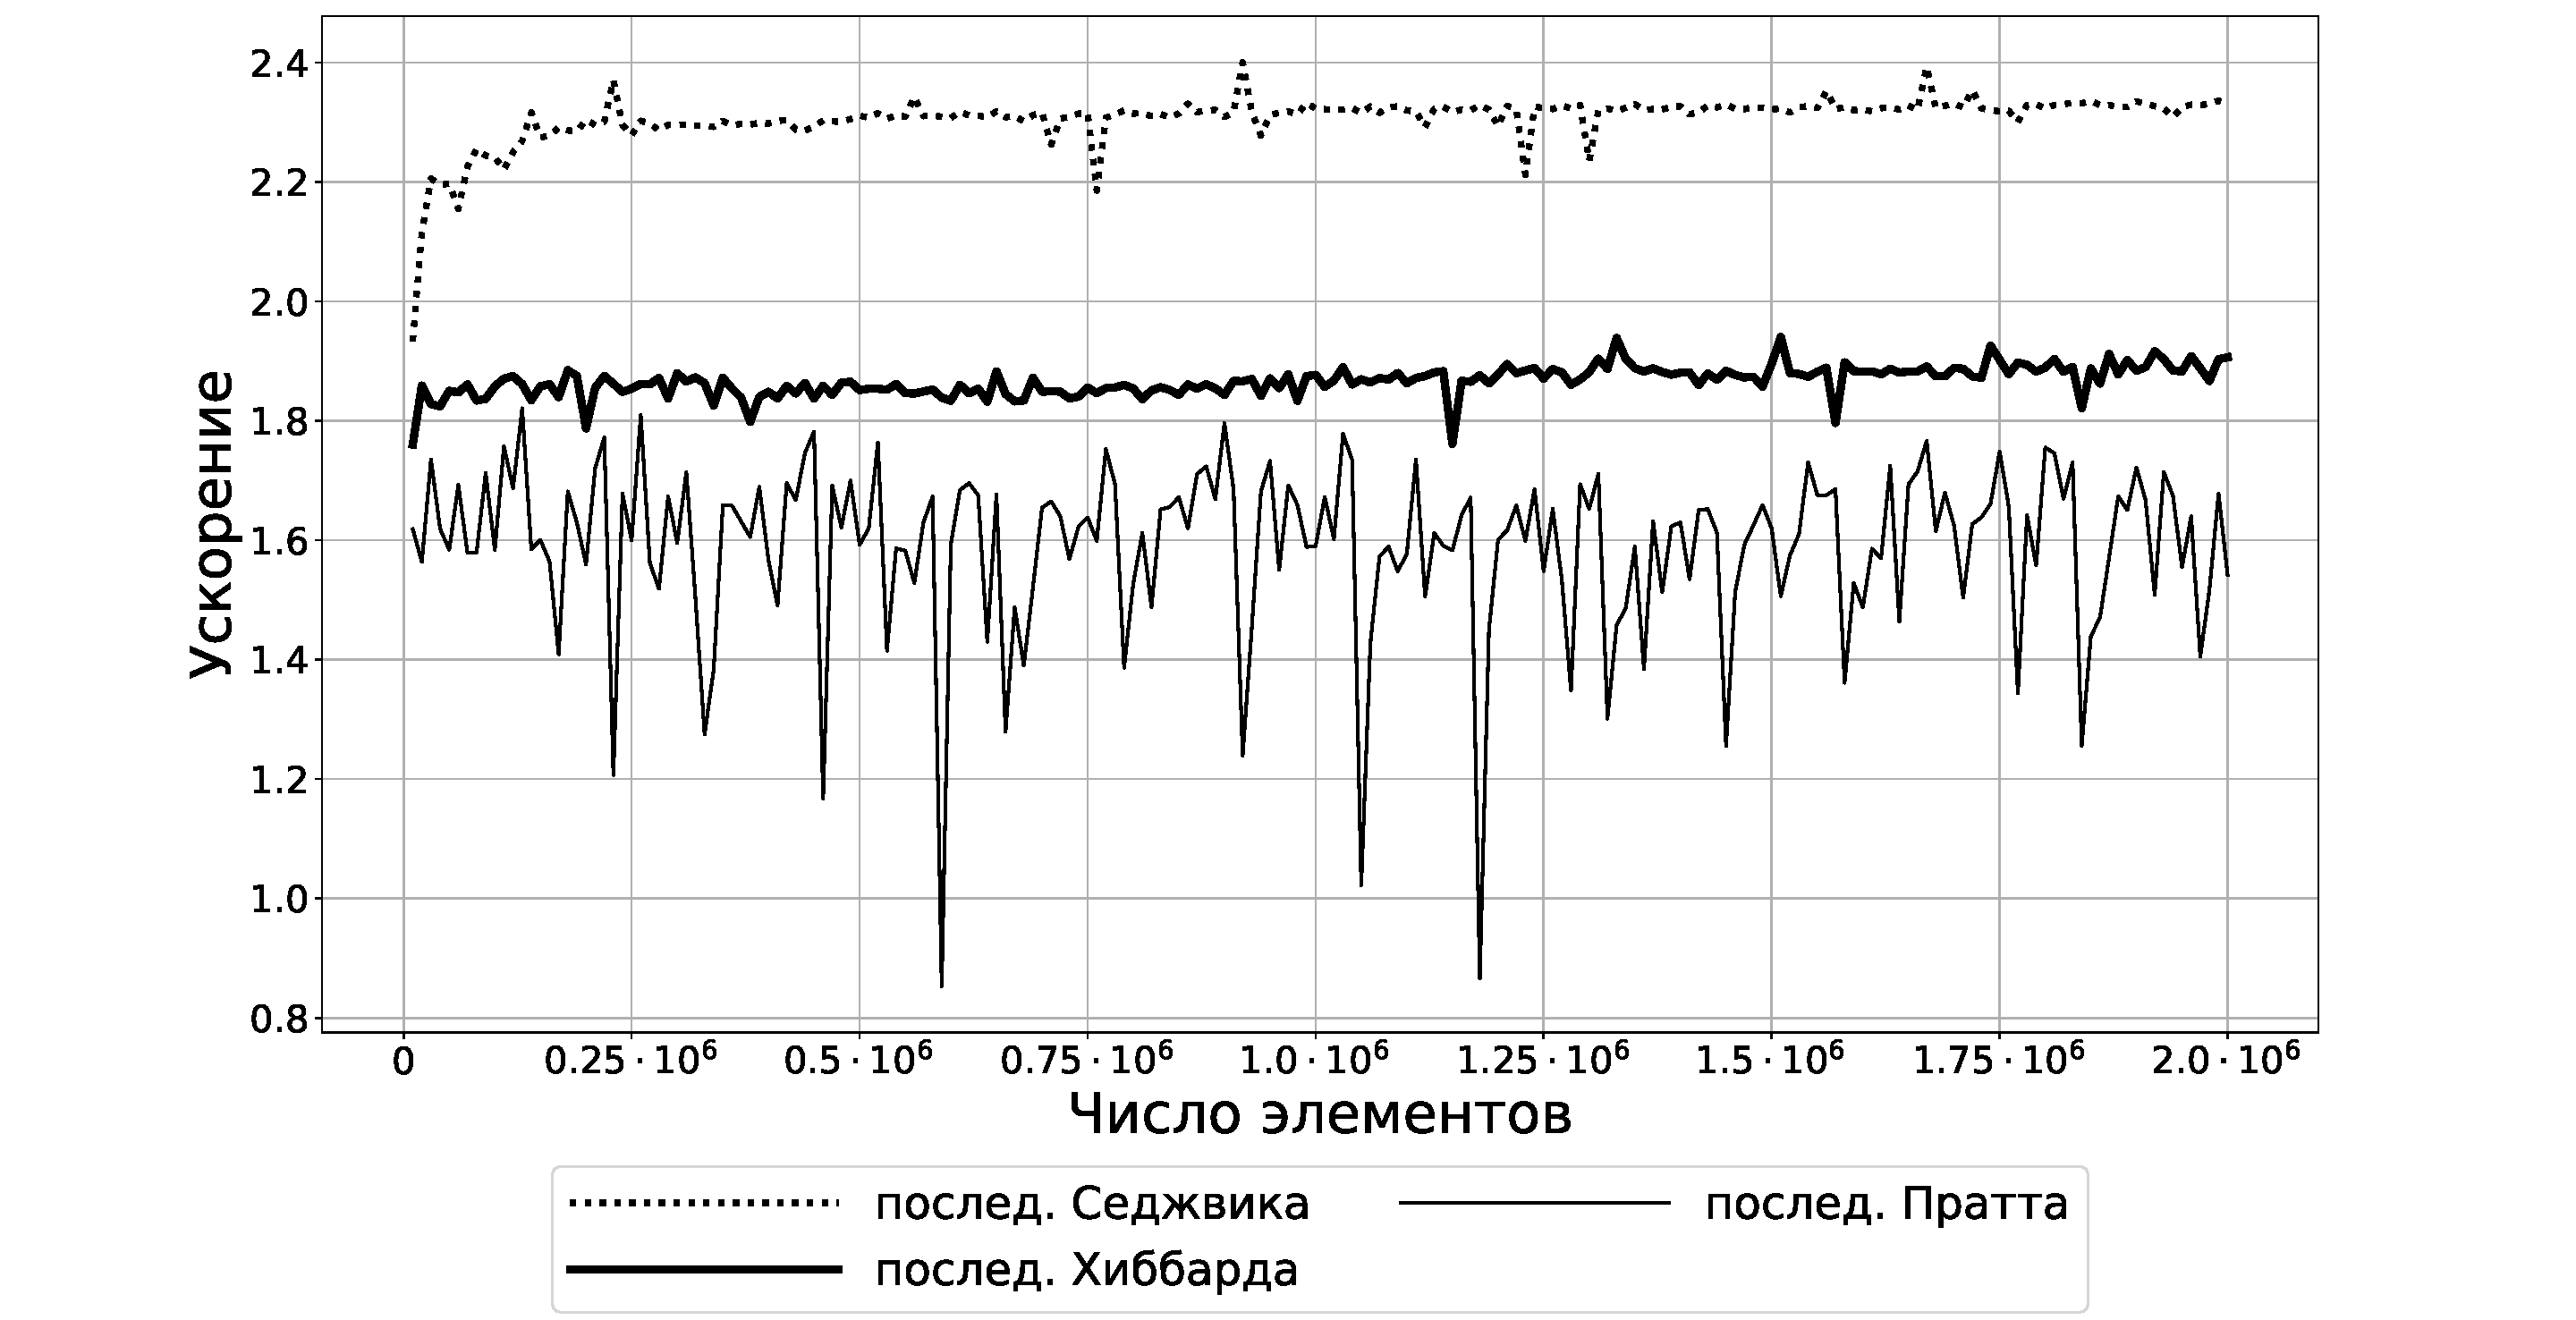
\includegraphics[width=1.0\textwidth]{./pics/text_4_vec_irreg/experimental_eff.pdf}
	\caption{Сравнение экспериментального ускорения векторизованной версии сортировки Шелла для различных последовательностей шагов.}
	\label{fig:text_4_vec_irreg_experimental_eff}
\end{figure}

Из графиков видно, что даже максимальное теоретическое ускорение далеко от идеальной верхней границы (которая равна 16 для значений типа float).
Экспериментальные же результаты ожидаемо оказываются еще ниже, и в конечном итоге финальное ускорение сортировки Шелла редко превышает отметку 2.

Проанализируем гистограммы распределения количества итераций внутреннего цикла для некоторых фиксированных значений $k$.
Из гистограмм, приведенных на рисунках \ref{fig:text_4_vec_irreg_shell_hist} и \ref{fig:text_4_vec_irreg_hibbard_hist} видно, что при переходе к векторизованной версии кода меняется характер распределения и количество выполнений внутреннего цикла с малым количеством итераций резко сокращается.

\begin{figure}[ht]
\centering
\begin{tabular}{ll}
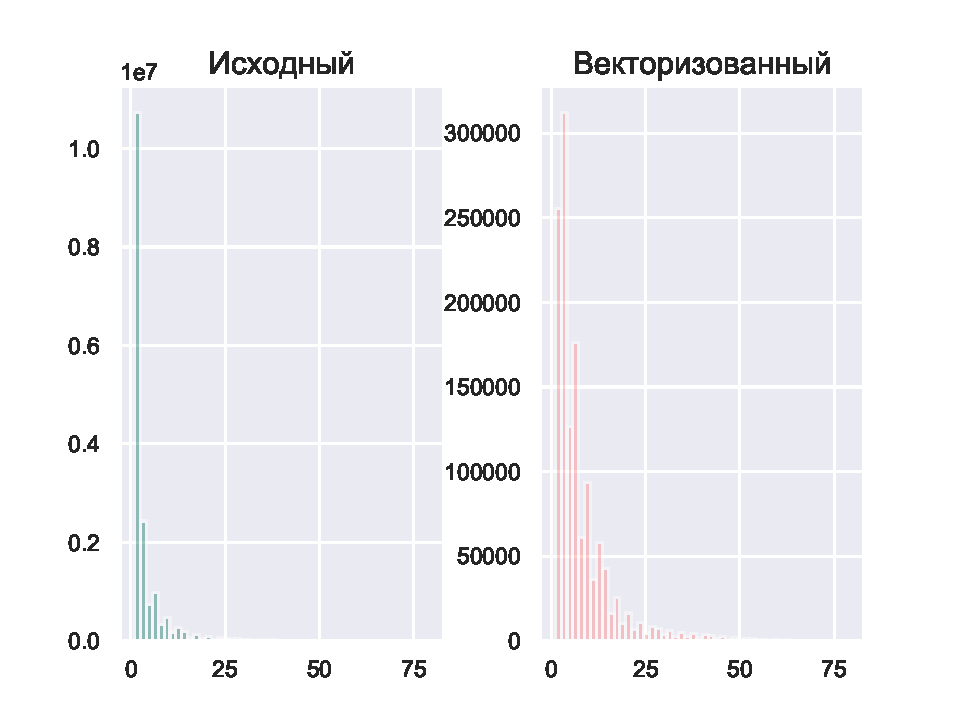
\includegraphics[scale=0.5]{./pics/text_4_vec_irreg/shell_k_4.pdf}
&
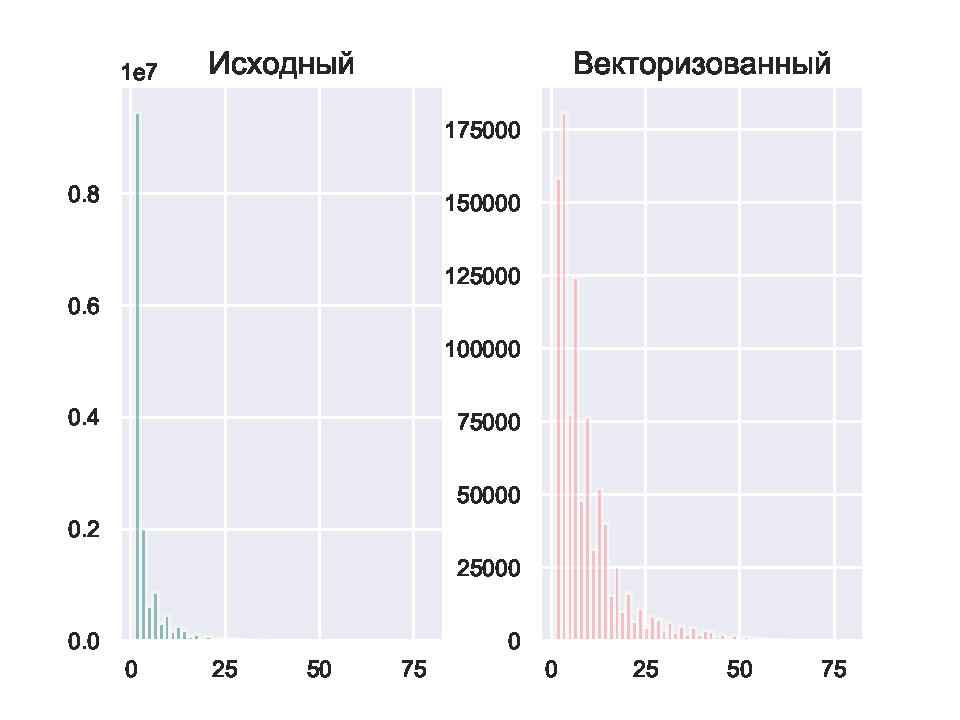
\includegraphics[scale=0.5]{./pics/text_4_vec_irreg/shell_k_15.pdf}
\end{tabular}
\caption{Гистограммы распределения количества итераций внутреннего цикла при сортировке с последовательностью
Шелла при $k = 4$ (слева) и $k = 15$ (справа) для скалярного и векторного кода.}
\label{fig:text_4_vec_irreg_shell_hist}
\end{figure}

\begin{figure}[h!]
\centering
\begin{tabular}{ll}
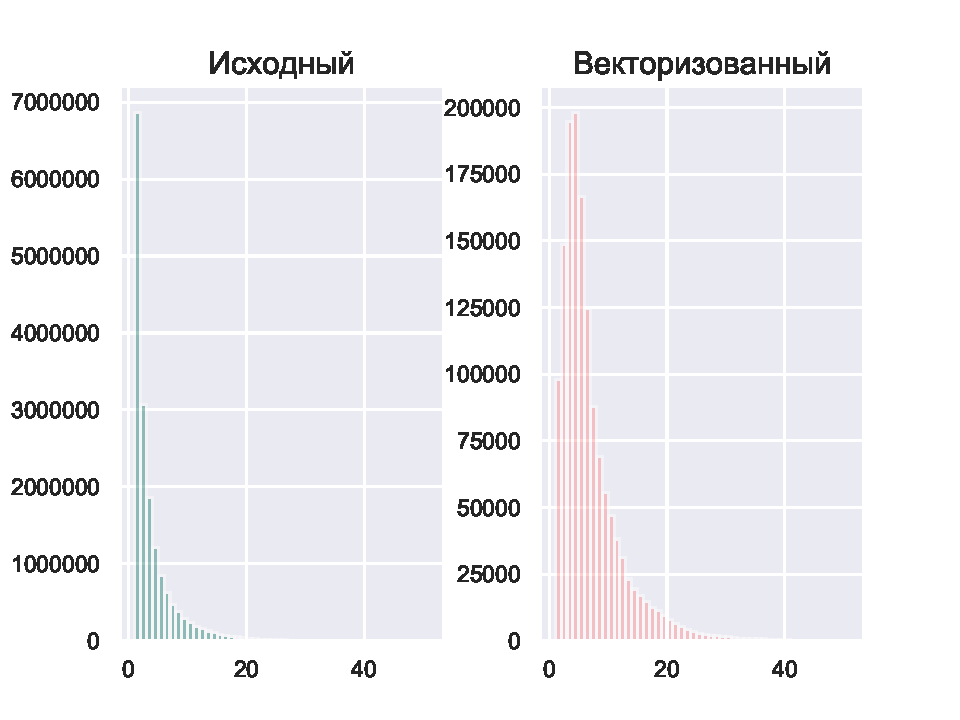
\includegraphics[scale=0.5]{./pics/text_4_vec_irreg/hibbard_k_3.pdf}
&
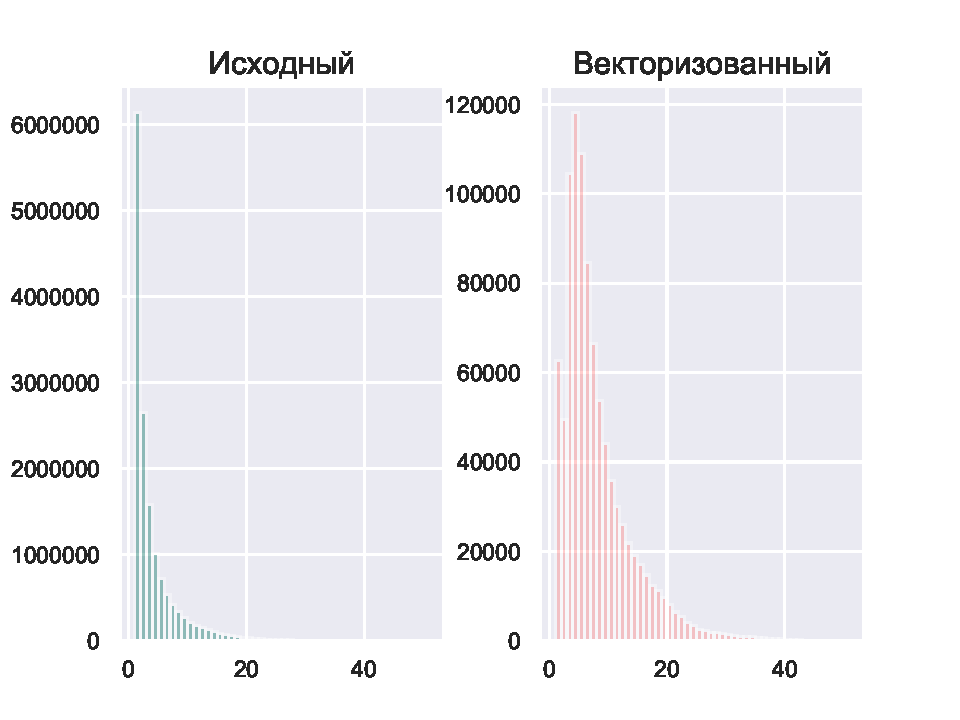
\includegraphics[scale=0.5]{./pics/text_4_vec_irreg/hibbard_k_15.pdf}
\end{tabular}
\caption{Гистограммы распределения количества итераций внутреннего цикла при сортировке с последовательностью
Хиббарда при $k = 3$ (слева) и $k = 15$ (справа) для скалярного и векторного кода.}
\label{fig:text_4_vec_irreg_hibbard_hist}
\end{figure}

Наличие только одной итерации внутреннего цикла в невекторизованной версии кода означает, что текущий рассматриваемый элемент \texttt{m[i]} уже стоит на своем месте в сортируемом срезе.
Для векторизованной версии одна итерация внутреннего цикла означает, что на своем месте стоят $w$ рассматриваемых элементов $w$ соседних одновременно сортируемых срезов, вероятность чего значительно ниже.
Таким образом, итерации внутренних циклов с малым количеством итераций растворяются в векторизованном коде, что снижает его производительность.

Теоретическая оценка эффективности векторизации с использованием последовательности Сэджвика оказалась ближе всего к экспериментальным результатам.
Это может быть объяснено тем, что последовательность шагов \texttt{ks} в данном случае достаточно короткая, и сортируемые срезы с разными значениями $k$ слабо коррелируют друг с другом.
В последовательности шагов Сэджвика присутствует только один шаг меньше 16 (это последний шаг $k = 1$), для всех остальных шагов доступно применение векторизации с максимальной плотностью.

Противоположностью последовательности Сэджвика является последовательность шагов Пратта, содержащая всевозможные шаги вида $2^i \cdot 3^j$.
Во-первых, эта последовательность очень длинная и содержит сразу 8 значений, которые меньше максимальной ширины векторизации, что негативно сказывается на производительности.
Во-вторых, срезы, индуцированные такими шагами, являются принципиально сильно коррелирующими, это приводит к нерегулярному снижению количества итераций во внутреннем цикле невекторизованной версии.
В итоге мы имеем очень непостоянный график как теоретического, так и и экспериментального ускорения, с низкой эффективностью векторизации и резкими провалами, опускающимися даже ниже единицы.
